%% packages
\documentclass{article}
\usepackage[a4paper, left=2.0cm, right=2.0cm, top=3.5cm]{geometry}
\usepackage[ngerman]{babel}
\usepackage{graphicx}
\usepackage{multicol}
\usepackage{amssymb}
\usepackage{titlesec}
\usepackage{wrapfig}
\usepackage{blindtext}
\usepackage{lipsum}
\usepackage{caption}
\usepackage{listings}
\usepackage{fancyhdr}
\usepackage{nopageno}
\usepackage{authblk}
\usepackage{amsmath} % tons of math stuff
\usepackage{mathtools} % e.g. alignment within matrix
%\usepackage{bm} % provides shorthand for bold in math mode
\usepackage{dsfont} % \mathds makes double stroke digits
\usepackage{esdiff} % provides \diff
%\usepackage[ISO]{diffcoeff}
\usepackage{xcolor}
\usepackage{csquotes} % e.g. provides \enquote
\usepackage[separate-uncertainty=true]{siunitx} % units
\usepackage{xcolor} % colored text
\usepackage{csvsimple}
\usepackage{subcaption}
\usepackage{physics}
\usepackage{hyperref}
\usepackage{nameref}
\hypersetup{colorlinks=true, linkcolor=black, pdfhighlight={/N}}
\usepackage{tcolorbox}
\usepackage{amsthm}
\usepackage{float}
\usepackage{enumitem}
\usepackage{booktabs}

% \sisetup{
%   scientific-notation = auto,  % Automatically use scientific notation for large/small numbers
%   output-exponent-marker = \text{e}  % (optional) for formatting the exponent symbol
% }

%\fancyhf[]{}

%% custom stuff
% own units
\DeclareSIUnit \VSS {\ensuremath{V_\mathrm{SS}}}
\DeclareSIUnit \VS {\ensuremath{V_\mathrm{S}}}
\DeclareSIUnit \Veff {\ensuremath{V_\mathrm{eff}}}
\DeclareSIUnit \Vpp {\ensuremath{V_\mathrm{pp}}}
\DeclareSIUnit \Vp {\ensuremath{V_\mathrm{p}}}
\DeclareSIUnit \VRMS {\ensuremath{V_\mathrm{RMS}}}
\DeclareSIUnit \ASS {\ensuremath{A_\mathrm{SS}}}
\DeclareSIUnit \AS {\ensuremath{A_\mathrm{S}}}
\DeclareSIUnit \Aeff {\ensuremath{A_\mathrm{eff}}}
\DeclareSIUnit \App {\ensuremath{A_\mathrm{pp}}}
\DeclareSIUnit \Ap {\ensuremath{A_\mathrm{p}}}
\DeclareSIUnit \ARMS {\ensuremath{A_\mathrm{RMS}}}

% change subsection numbering to capital letters
\newcommand{\subsectionAlph}{ \renewcommand{\thesubsection}{\arabic{section}.\Alph{subsection}} }
% change subsection numbering to lowercase letters
\newcommand{\subsectionalph}{ \renewcommand{\thesubsection}{\arabic{section}.\alph{subsection}} }
% change subsubsection numbering to lowercase letters
\newcommand{\subsubsectionalph}{ \renewcommand{\thesubsubsection}{\arabic{section}.\arabic{subsection}.\alph{subsubsection}} }
% own fig. that works with multicols
\newenvironment{Figure}
  {\par\medskip\noindent\minipage{\linewidth}}
  {\endminipage\par\medskip}
\newcommand*{\inputPath}{./plot} % prepend this command to the argument of all input commands
\graphicspath{ {./images/}{./figure/}{../plot/}{../../plot/}{../../latex/assets/}{./assets/} }
% own enviroment for definitions
\newenvironment{definition}[1]
{\begin{quote} \noindent \textbf{\textit{#1\ifx&#1& \else : \fi}} \itshape}
{\end{quote}}



% own commands
% \newcommand{\rarr}{$\to\,$} %A$\,\to\,$B
\newcommand{\defc}{black}
\newcommand{\colorT}[2][blue]{\color{#1}{#2}\color{\defc}}
\newcommand{\redq}{\color{red}(?)\color{\defc}}
\newcommand{\question}[1]{\colorT[purple]{\textbf{(#1)}}}
\newcommand{\todo}[1]{\colorT[red]{\textbf{(#1)}}}
\newcommand{\mr}{\mathrm}


%% preparation


%dachte wir können hier durchführung und gleich Auswertung der einzelnen Versuchsaufgaben schreiben und im Fazit ein gesamtfazit

%\displaystyle \lim_{x \to \infty}

\begin{document}
    \title{Elektronikpraktikum \\ \textbf{Versuch 0: Einführung und Vorversuch}}
    \author[1]{Carlos Pascua \thanks{s87cpasc@uni-bonn.de}}
    \author[1]{Anna Maróti\thanks{s32amaro@uni-bonn.de}}
    \author[1]{Cornelius Heiming\thanks{s64cheim@uni-bonn.de}}
    \affil[1]{Uni Bonn}
    %\date{\today}
	\pagenumbering{gobble}
    \begin{titlepage}
     \maketitle   
    \end{titlepage}
        

\tableofcontents
\newpage
\pagenumbering{arabic}

\pagestyle{fancy}
\fancyhead[R]{\thepage}
\fancyhead[L]{\leftmark}

\section{Theorie}

\subsection*{Einführung}
In diesem Versuch wurde der Umgang mit  relevanten Geräten des Elektronikpraktikums geübt, 
indem verschiedene Signaltypen eines Funktionsgenerators analysiert wurden. 
Im Anschluss wurde die Anstiegszeit eines Rechtecksignals bestimmt. 


\subsection*{Signalquellen}
\begin{itemize}
    \item Spitze-Spitze $U_{SS} $in$ V_{SS}$ oder $U_{pp} $in$ V_{pp}$: Die Differenz zwischen den niedrigsten und höchsten Spannungswert des Signals.
    \item Spitzenwert $U_{S}$in$ V_{S}$ oder $U_{p}$in$ V_{p}$: Maximalwert der auftretender Spannung 
    \item Effektivwert $U_{eff}$ : ist gleich der Spannung, die bei einer konstanten Gleichspannung und einem Ohmschen Widerstand die gleiche mittlere Leistung $P$ liefert. $U_{eff}= \sqrt{\langle U^2(t) \rangle}$
\end{itemize}


\subsection*{Das Oszilloskop}

Das Oszilloskop, ein elektronisches Messgerät mit welchem zeitabhängige Signale dargestellt werden können, besteht aus den folgenden Bauteilen
\begin{itemize}
    \item Netzteil
    \item Elektronenstrahlröhre: bestehend aus einem Glaskolben mit einer Glühkathode und einer Lochanode,
     die sich innerhalb eines Wehneltzylinders befinden (1). Zwischen Kathode, woraus Elektronen emittiert
      werden, und der Lochanode herrscht ein elektrsches Feld, wodurch die Elektonen zur Anode beschleunigt 
      werden. Danach geht der gebündelte Elektronenstrahl durch zwei weiteren Elektroden mit elektrischen 
      Feldern(2) wodurch er weiter abgelenkt wird. Schließlich trifft der Strahl (4) auf einen Leuchtschirm
       (3), auf dem er als leuchtender Punkt (5) sichtbar wird \ref{fig:elektronenstrahlröhre} \\
        %ich muss die Einstellung raussuchen, wo ich hyperlink machen kann für die Bilder, damit da nicht so eine lonly 1 steht
    
    \item y-Verstärker: ein Breitbandverstärker
    
    \item Zeitablenkeinheit: Um ein stehendes Bild einer periodischen Spannung zu erhalten, wird mit einem Sägezahn-Signal am zweiten Elektrodenpaar eine Spannung angelegt. Hierdurch bewegt sich der Strahl mit konstanter Geschwindigkeit über den Leuchtschirm. Damit ein Bild entstehen kann muss noch die Bedingung erfüllt werden, dass die Frequenz der Messspannung ein ganzzahliges Vielfaches der Kippfrequenz ist.

    
\end{itemize}
\begin{figure}[H]
    \centering
    \includegraphics[width=0.7\textwidth]{figs/Versuch0_Elektrodenstrahlröhre.png}
    \caption{Aufbau eines Elektronenstrahlröhres \cite{anleitung}}
    \label{fig:elektronenstrahlröhre}
\end{figure}

\subsection*{Bandbreite}
Die Bandbreite wird durch einen RC-Tiefpass begrenzt, welches die hohen Frequenzen vollständig dämpft.
\begin{align}
  B = f_{grenz}= \frac{1}{2\pi RC}=  \frac{1}{2\pi \tau}
\end{align}
Hier entspricht $R$ dem Ohmschen Widerstand und $C$ ist die Kapazität des Kondensators. 

\subsection*{Anstiegszeit}
Bei einem realen Rechtecksignal weist der Spannungsverlauf eine endliche Anstiegszeit $\Delta t$
 auf, bevor das Signal seinen Maximalwert erreicht. Die Anstiegszeit ist definiert als der
  Zeitraum zwischen  $t(0,9\cdot U_{max}- 0,1\cdot U_{max})$, also die Zeit des Spannungsantiegs 
  von 10$\%$ auf 90 $\%$(\autoref{fig:anstiegzeit}).
Dieser gemessene Wert setzt sich aus dem theoretischen Wert der Anstiegszeit und dem 
Anstiegszeit das Oszilloskops folgendermaßen zusammen:

\begin{equation}
    \Delta t_{gemessen}^2 = \Delta t_{signal}^2 + t_{Oszi}^2
\end{equation}
wobei für den Oszilloskop gilt: $B \cdot \Delta t = 0,35$
\begin{figure}[H]
    \centering
    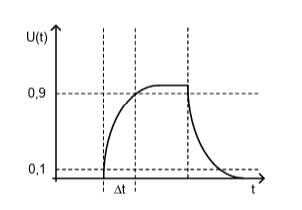
\includegraphics[width=0.5\textwidth]{figs/Verusch0_Anstiegszeit.png}
    \caption{Anstiegszeit eines Rechtecksignals\cite{anleitung}}
    \label{fig:anstiegzeit}
\end{figure}
\newpage 

\section{Voraufgaben}

\subsection*{Aufgabe A}
Folgende Größen gelten für die Spannung $U(t)= U_0 \cdot \sin{(\omega t)}$ :\\
\\
Spitze-Spitze-Spannung: \begin{equation}
        U_{SS}= 2 \cdot U_0
    \end{equation}
Spitzenspannung: 
    \begin{equation}
        U_{S}= U_0
    \end{equation}
 Effektivspannung:
    \begin{align*}
        U_{eff} &= \sqrt{ \langle U_0 ^2 \sin{(\omega t)}^2 \rangle}
        = \sqrt{ U_0 ^2 \langle \sin{(\omega t)}^2 \rangle} = \frac{U_0}{\sqrt{2}}
    \end{align*}
wobei $\langle \sin{(\omega t)}^2 \rangle = \frac{1}{2}$ ist.



\subsection*{Aufgabe B}
Der Effektivwert eines symmetrischen Rechtecksignals mit $U_S= 10 V$ entspricht:

\begin{equation}
    U_{eff}= \sqrt{\langle U_0 ^2 \rangle}= \sqrt{\langle U_S ^2 \rangle}= U_S = 10V
\end{equation}

\subsection*{Aufgabe C}

\begin{figure}[H]
    \centering
    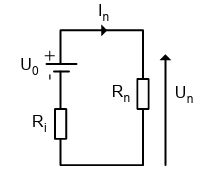
\includegraphics[width=0.4\textwidth]{figs/Versuch0_Ersatzbild.png}
    \caption{Ersatzschaltbild der Generator-Spannungsquelle\cite{anleitung}}
    \label{fig:Ersatzbild}
\end{figure}

Für die Bestimmung des Innenwiderstandes des Generatorausgangs, kann die Spannung zunächst so ausgedrückt werden:
\begin{equation}
\label{Gl 1}
    U_n = U_0 \frac{R_n}{R_n + R_i}
\end{equation}
wobei $R_i$ der Innenwiderstand ist. Dieses kann zu folgender Formel umgestellt werden: 
\begin{equation*}
    U_0 = \frac{U_n \cdot (R_n +R_i)}{R_n}
\end{equation*}

Dann gilt die Formel für zwei unterschiedliche Widerstände:
\begin{equation*}
   U_1 \cdot \biggl(1 +\frac{R_i}{R_1}\biggr) = U_2 \cdot \biggl(1 +\frac{R_i}{R_2}\biggr) 
\end{equation*}
\begin{equation*}
    \Leftrightarrow U_1 + R_i \cdot \biggl(\frac{U_1}{R_1}\biggr) = U_2 + R_i \cdot \biggl(\frac{U_2}{R_2}\biggr)
\end{equation*}
Mit der  $I= \frac{U}{R}$ folgt: 
\begin{equation*}
    \Leftrightarrow U_1 +I_1 \cdot R_i =  U_2 +I_2 \cdot R_i
\end{equation*}
\begin{equation*}
    \Leftrightarrow R_i \cdot (I_1-I_2) = U_2 -U_1
\end{equation*}
\begin{equation}
\label{Gl 6}
    \Leftrightarrow R_i = \frac{U_2 - U_1}{I_1 - I_2}
\end{equation}
Anhand dieser Formel und den folgenden Angaben aus dem Skript kann der Wert des Innenwiderstands berechnet werden: \\
Maximalamplitude ohne Belastung: $U_\mathrm{1} = 20V_\mathrm{SS}$. \\
Maximalamplitude bei einer Belastung von $R = 50 \Omega$: $U_\mathrm{2} = 10V_\mathrm{SS}$. \\
Der Spitze-Spitze Wert für den Strom ist: $I_1 = 0A_{SS}$ und $I_2 = 0,2 A_{SS}$. Jetzt kann man \autoref{Gl 6} benutzen.
\begin{equation*}
    R_i = \frac{20-10}{0,2-0} = 50 \Omega
\end{equation*}



%!!!!!!!!!!Woher die werte? sind sie noch gleich?

\subsection*{Aufgabe D}
Anordnung des Oszilloskops wurde studiert und sich über die Funktion der Elemente aufgeklärt. 

\subsection*{Aufgabe E}
\label{subsec:afgE}
Folgender Zusammenhang wird für den Tiefpass geprüft:  $B\cdot \Delta t = 0,35$.\\
Bei Tiefpassfilter gilt für die Bandbreite: 
\begin{equation}
    B = f_{grenz} = \frac{1}{2\pi RC} = \frac{1}{2\pi \tau}
\end{equation}
Die Anstiegszeit entspricht:
 \begin{equation*}
     \Delta t = (ln(0,9)-ln(0,1))\cdot \tau 
 \end{equation*}
Also erhält man die folgende Formel:
 \begin{equation*}
     \iff B = \frac{1}{2\pi \tau} \cdot (ln(0,9)-ln(0,1))\cdot \tau 
 \end{equation*}
 \begin{equation*}
     \iff B = \frac{ln(0,9)-ln(0,1)}{2 \pi} \approx 0,35
 \end{equation*}
 Also entspricht dieses dem genannten Zusammenhang.

 \section{Versuchsaufbau, -durchführung, Messwerte und Auswertung}
 \subsection*{Bestimmung der Anstiegszeit des Oszillographen}
     \begin{figure}[H]
         \centering
         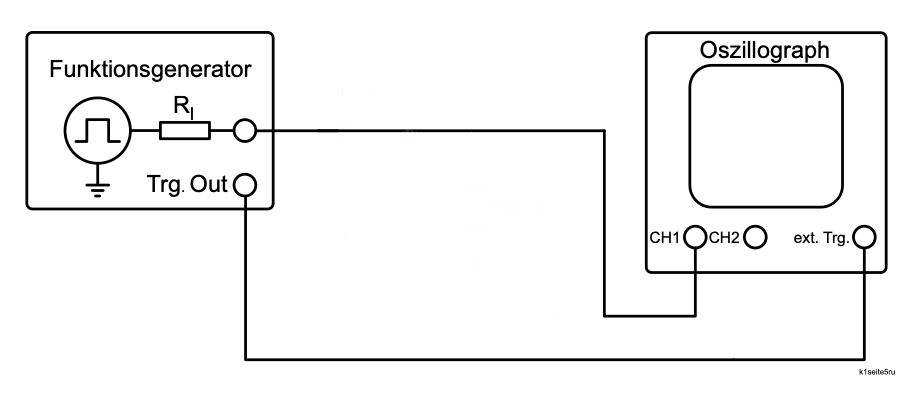
\includegraphics[width=0.8\textwidth]{figs/Aufbau_0_1_Oszilloskop.png}
         \caption{Schaltplan Funktionsgenerator und Oszilloskop~\cite{anleitung}}
         \label{fig:aufbau_0_1_oszilloskop.png}
     \end{figure}
     \begin{enumerate}[label=\alph*]
         \item In dieser Aufgabe soll der Oszillograph untersucht werden. Dafür wird der Generatorausgang mit dem CH1 Eingang des Oszilloskops mittels eines Koaxialkabels verbunden. Nach dem Triggern konnten verschiedene Oszillogramme beobachtet werden.
         
         \begin{figure}[H]
    \centering
    \begin{subfigure}[b]{0.48\textwidth}
        \centering
        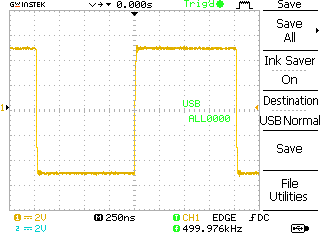
\includegraphics[width=\textwidth]{MesswerteVersuch0/A0000DS.png}
        \caption{Rechtecksignal}
        \label{fig:A0000DS}
    \end{subfigure}
    \hfill
    \begin{subfigure}[b]{0.48\textwidth}
        \centering
        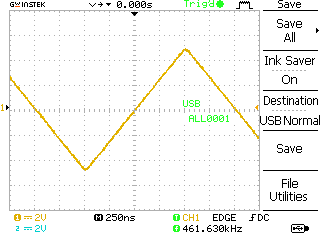
\includegraphics[width=\textwidth]{MesswerteVersuch0/A0001DS.png}
        \caption{Dreieckssignal}
        \label{fig:A0001DS}
    \end{subfigure}
    \vskip\baselineskip
    \begin{subfigure}[b]{0.48\textwidth}
        \centering
        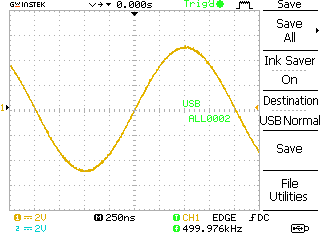
\includegraphics[width=\textwidth]{MesswerteVersuch0/A0002DS.png}
        \caption{Sinussignal}
        \label{fig:A0002DS}
    \end{subfigure}
    \caption{Verschiedene Signalformen}
    \label{fig:alle_signale}
\end{figure}


         Rechtecks-, Dreiecks- und Sinussignal konnten erfolgreich eingestellt werden. Hiermit konnten die Zusammenhänge der Amplitude und Frequenz des Funktiongenerators im Zusammenhang mit dem Bild des Oszillogramms untersucht werden. Die eingestellte Amplitude entspricht $U_S$ im Oszillographen auf der y-Achse und die Frequenz beeinflusst antiproportional die Darstellung auf der x-Achse (je höher die Frequenz desto gestauchter ist das Signal).

         \item Danach wird ein Rechtecksignal mit einer Frequenz von $\SI{2}{\mega\hertz}$ und einer Amplitude von beispielsweise $\SI{1}{\volt}$ eingestellt. Die Anstiegszeit $\Delta t_\mathrm{gemessen}$ wird bestimmt, indem die Zeitdifferenz zwischen dem Zeitpunkt, an dem $U(t)$ den Wert $0.1 U_0$ erreicht, und dem Zeitpunkt, an dem $U(t)$ den Wert $0.9 U_0$ erreicht, gemessen wird.

         \begin{figure}[H]
             \centering
             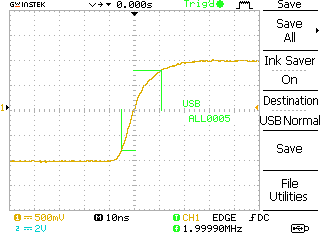
\includegraphics[width=0.7\textwidth]{MesswerteVersuch0/A0005DS.png}
             \caption{Rechteckssignalanstieg (detailliert)}
             \label{fig:A0005DS}
         \end{figure}
         Aus der Grafik \ref{fig:A0005DS} wurde die Anstiegszeit $\Delta t_\mathrm{gemessen}$ abgelesen. Dafür wurden die $10\%$ und $90\%$ markiert und damit die Zeitpunkte ermittelt, an denen die Spannung $U(t)$ den Wert $0.1 U_0$ und $0.9 U_0$ erreicht. Die Anstiegszeit $\Delta t_\mathrm{gemessen}$ betrug dann $\SI{16}{\nano\second}$ (Genau $8$ Einheiten der Skala, die je $\frac{1}{5}$ von $\SI{10}{\nano\second}$ sind). Der Messfehler betrug $\Delta(\Delta t_\mathrm{gemessen}) =  \SI{1}{\nano\second}$. Der Betriebsanleitung des Oszilloskops \cite{anleitung} zufolge beträgt die Bandbreite des Oszilloskops $B = \SI{50}{\mega\hertz}$\cite{oszibedienungsanleitung}. Daraus folgt mit der Formel $B \cdot \Delta t = \SI{0.35}{}$ (siehe Voraufgabe~\ref{subsec:afgE}) die Anstiegszeit:
         \begin{align*}
             \Delta t_\mathrm{Oszi} = \frac{0.35}{\SI{50}{\mega\hertz}} = \SI{7}{\nano\second}
         \end{align*}
         Für die Anstiegszeit des Signals $\Delta t_\mathrm{Signal}$ gilt nach der Anleitung\cite{anleitung} die Näherung:
         \begin{align*}
             (\Delta t_\mathrm{Signal})^2 &= (\Delta t_\mathrm{Oszi})^2 - (\Delta t_\mathrm{gemessen})^2 \\
             \Delta t_\mathrm{Signal} &= \sqrt{(\Delta t_\mathrm{Oszi})^2 - (\Delta t_\mathrm{gemessen})^2} \\
             &= \sqrt{(\SI{16}{\nano\second})^2 - (\SI{7}{\nano\second})^2} \approx \SI{14.39}{\nano\second}
         \end{align*}
         Mittels Gaußscher Fehlerfortpflanzung ergibt sich:
         \begin{align*}
             \Delta(\Delta t_\mathrm{Signal}) &= \frac{2 t_\mathrm{gemessen}}{\sqrt{(\Delta t_\mathrm{gemessen})^2 - (\Delta t_\mathrm{Oszi})^2}} \cdot \Delta(\Delta t_\mathrm{gemessen}) \\
             &= \frac{2 \SI{16}{\nano\second}}{\sqrt{(\SI{16}{\nano\second})^2 - (\SI{7}{\nano\second})^2}} \cdot \SI{1}{\nano\second} \\
             &\approx \SI{2.3}{\nano\second}
         \end{align*}
         Also ergibt sich für die Anstiegszeit des Signals:
         \begin{align*}
             \Delta t_\mathrm{Signal} &= \SI{14.4}{\nano\second} \pm \SI{2.3}{\nano\second}
         \end{align*}

         Hiermit lässt sich die Bandbreite des Funktionsgenerators bestimmen:
        
        \begin{align*}
            B &=
            \frac{0.35}{\Delta t_\mathrm{Signal}}\\
            &=\frac{0.35}{\SI{14.4}{\nano\second}} \approx \SI{24.3}{\mega\hertz}\\
            \Delta B &= \frac{0.35}{(\Delta t_\mathrm{Signal})^2} \cdot \Delta (\Delta t_\mathrm{Signal})\approx \SI{3.9}{\mega\hertz}\\
        \end{align*}
        
        Also entspricht die Bandbreite des Funktiongenerators $B = \SI{24.3 \pm 3.9}{\mega\hertz}$. Somit hat der experimentell bestimmte Wert eine totale Abweichung von etwa $50\%$ von dem Literaturwert von  $50MHz$(\cite{oszibedienungsanleitung}). Mögliche Messunsicherheiten konnten entstanden sein, bei der Ablesung und Bestimmung der Anstiegzeit. Aber auch systematische Fehler können eine große Rolle gespielt haben, da die Länge der Kabel und deren Alter das Signal bisschen verfälschen können, wodurch die Unsicherheit größer wurden.
        
        
        
        
        

         \item Zuletzt wurde der Generatorausgang mit einem Tiefpass verbunden. Es sollte eine 
         Zeitkonstante von $\tau = \mathcal{O}(\SI{10}{\micro\second} \text{ bis } \SI{100}{\micro\second})$ realisiert werden, also wurde 
         bspw. $R = \SI{22}{\kilo\ohm}$ und $C = \SI{1}{\micro\farad}$ gewählt. 
         Der Tiefpass wird erneut mit dem CH1-Eingang des Oszilloskops verbunden. 
         Der Generator wird auf ein Sinus-Signal mit 10 verschiedenen Frequenzen eingestellt, die 
         für die Messung sinnvoll sind.  
         Dabei wird sich jeweils die Amplitude am Signalgenerator notiert und in einer Tabelle aufgetragen. 

         Die Grenzfrequenz berechnet sich zu:
         \[
         f_{\text{grenz}} = \frac{1}{2\pi R C} = \frac{1}{2\pi \cdot \SI{1}{\micro\farad} \cdot \SI{22}{\kilo\ohm}} 
         \approx \SI{7.24}{\kilo\hertz}
         \]
         Mit unseren Grenzfrequenz ist der Punkt, ab das Signal abgedämpft wird, gefunden und daraus 
         werden die Messpunkte ausgewählt. 
         \begin{table}[H]
            \centering
            \begin{tabular}{|c|c|}
            \hline
            $\omega$ [kHz] & $U_{\text{pp}}$ [V] \\
            \hline
            6.5  & 2.85 \\
            6.7  & 2.81 \\
            7.0  & 2.75 \\
            7.05 & 2.75 \\
            7.1  & 2.74 \\
            7.15 & 2.74 \\
            7.2  & 2.73 \\
            7.22 & 2.72 \\
            7.24 & 2.71 \\
            7.26 & 2.70 \\
            7.31 & 2.70 \\
            7.61 & 2.65 \\
            8.0  & 2.60 \\
            10.0 & 2.25 \\
            50.0 & 0.59 \\
            100.0 & 0.31 \\
            \hline
            \end{tabular}
            \caption{Messwerte von $\omega$ und $U_{\text{pp}}$}
            \label{tab:omega_upp}
            \end{table}
            Nun werden die berechnete Dämpfung in $dB$ gegen die Frequenz aufgetragen und erhält man 
            den folgenden Graphen bzw. ein sogennates $BODE-$Diagramm. 

         \begin{figure}[H]
             \centering
             \includegraphics[width=0.8\textwidth]{figs/versuch0_1c_korrekt}
             \caption{Dämpfungsplot}
             \label{0_1_(c)_Dämpfung}
         \end{figure}

        Wie man aus der Grafik erkennen kann, die Mehrheit der gewählten Messpunkten waren nah zu dem 
         berechneten Grenzfrequenz, damit diese experimentell bestätigt werden kann. Aus diesem Grund sind mehrere Messwerten am Anfang des Graphens. Die erwartete Kurve ist aber trotzdem zu erkennen und man sieht, dass höhere Frequenzen mehr gedämpft werden, nachdem die Grenzfrequenz erreicht wurde.  
         
         
         \begin{figure}[H]
             \centering
             \includegraphics[width=0.8\textwidth]{figs/versuch0_1cdet_korrekt}
             \caption{Dämpfungsplot in detaillierten Ansicht}
             \label{0_1_(c)_Dämpfung_detail}
         \end{figure}
         
         Wenn man nun die Dämpfungskurve im Bereich der Grenzfrequenz näher betrachtet, kann man anhand der $-3dB$ Linie den experimentellen Grenzfrequenz ablesen. In diesem Fall liegt er geschätzt bei $f_{\text{grenzE}} \approx  10^{0.84} \approx\SI{6.8 \pm 0.1}{\kilo\hertz}$. 
         
        Somit ergibt sich eine absolute Abweichung von etwa $6 \% $. Diese Abweichung könnte aus verschiedenen Quellen entstanden sein. Einerseits haben die benutzen Widerstände und Kondensatoren eigene Fehler, weshalb die der theoretisch errechnete Wert auch nur eine Approximierung ist. Des Weiteren wurde mit realen Materialien gearbeitet, wo man systematische Fehler nicht ausschließen kann.
         
        \end{enumerate}

        \section{Fazit bzw. Resultat}
        
        
        In diesem Versuch wurden anhand eines Funktionsgenerators die Arbeit mit einem Oszilloskopen geübt. 
        Hierzu wurde die realistische Anstiegszeit von einem Rechtecksignal 
        $\Delta t_\text{Signal} = \SI{14.4 \pm 2.3}{\nano\second}$
         und die Bandbreite $B = \SI{24.3 \pm 3.9}{\mega\hertz}$ für den Funktionsgenerator bestimmt, welches etwa nur $50\%$ des zu erwarteten Wertes entsprach.
         Des weiteren wurde ein Bode-Plot für einen Tiefpass aufgenommen, welches den Erwartungen entsprach, da es 
         zeigte, dass hohe Frequenzen stärker gedämpft wurden. Anhand des Graphens wurde noch die Grenzfrequenz des 
         Tiefpasses auf $f_{\text{grenzE}} \approx \SI{6.8 \pm 0.1}{\kilo\hertz}$ bestimmt, welches eine totale Abweichung
           $6 \% $ von dem errechneten Wert $ f_{\text{grenz}}
         \approx \SI{7.24}{\kilo\hertz}$ besaß.


        \begin{thebibliography}{9}

        \bibitem{anleitung}
        \textit{Elektronikpraktikum -- Versuchsbeschreibungen}, Universität Bonn, 04.04.2025


\end{thebibliography}

\end{document} 